
	\citep{asano2008efficient} ont exploité les propriétés du graphe du web pour présenter une nouvelle méthode de compression (ECWG) sans perte permettant d'extraire les motifs à partir de la matrice d'adjacence. Il proposent un vocabulaire composée de six types de blocs (Motifs): un bloc horizontale de 1, un bloc verticale de 1, un bloc diagonale de 1, un rectangle de 1, un bloc de 1 sous forme de L et le singleton 1. Avant de procédé à l'extraction des motifs, la liste d'adjacence du graphe est partitionner selon les hôtes. Une nouvelle matrice d'adjacence est donc construite pour chaque hôte contenant les liens existants entre ses pages aux quel les liens inter-hote sont concaténés.
					Les blocs B sont détectés par la suite et chacun est représenté par un quadruplets (i, j, type(B), dim(B)) où i,j représentent les coordonnées du premier élément du blocs dans la matrice d'adjacence de l'hôte, type(B) représente le type du bloc et dim(B) représente les dimensions du bloc (omis dans le cas du singleton). 
					\begin{figure}[h]
					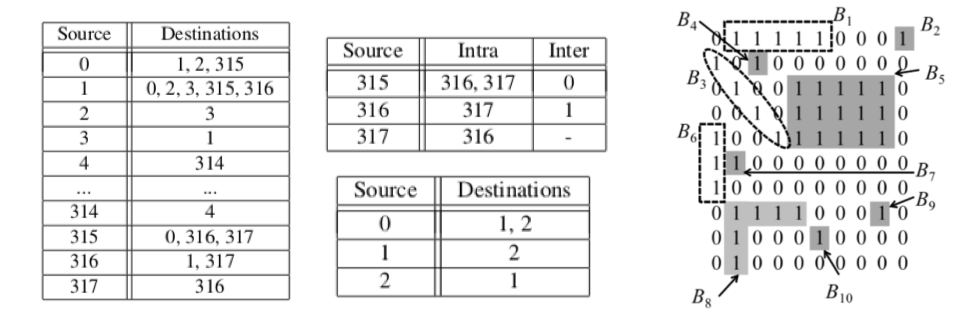
\includegraphics[scale=0.5]{ressources/image/inter_intra.png} 
					\caption{Exemple illustrant le principe de fonctionnement \citep{asano2008efficient}}
					\label{interIntra}
				\end{figure}